\section{Evaluation}
\label{sec:evaluation}
The performance of the DCG-UPUP-Away model is demonstrated in two experiments.
First, a simulated turtlebot within randomly generated simulated environments is given a series of user-generated natural language commands.
Second, an actual turtlebot is given specific commands in a laboratory environment in order to demonstrate novel behaviors enabled by the DCG-UPUP-Away model.
Both experiments assume a perfect object recognizer that translates the raw sensor data into a world model $\Upsilon$ that can be used by the DCG-UPUP-Away model, as well as an initial set of hand-labeled training examples for training the LLM to ground cubes, spheres, and cylinders.
In all trials, training the model with $53$ positive examples took less than $1$ minute on a Lenovo Thinkpad X1 Carbon, and grounding a command took under $40$ seconds.
\subsection{Experimental Setup}
The simulated testing environments are randomly generated in Gazebo.
Ten worlds are created, and each is populated with a random collection of objects in randomized locations.
There are $8$ possible object types (including cubes, spheres, and cylinders) in $3$ possible colors, for a total of $24$ objects.
Each object has a $15\%$ chance of being added to a given map.
Using such a procedure to generate environments coupled with the limited field of view of the turtlebot has caused $87\%$ of the objects to be placed outside the initial field of view of the robot, which demonstrates the need for the ability to ground commands to hypothesized objects.

After generating the 10 worlds, the screenshots of a world with a highlighted single object are uploaded to Amazon Mechanical Turk. For each image, the users were instructed to write a command ``for approaching the highlighted object.''
These image-command pairs were saved for evaluating whether a robot, when placed in the corresponding simulated world and given the natural language command, successfully approaches the correct object.
An example screenshot, with an annotation supplied by a user, is shown in Fig.~\ref{fig:amt}.
\begin{figure}[h]
	\centering
    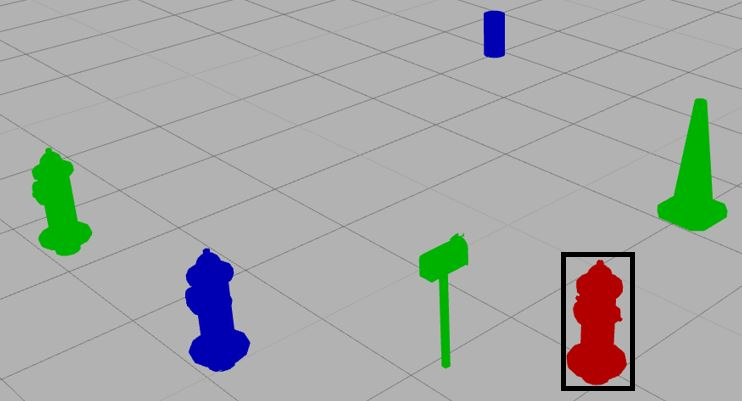
\includegraphics[width=7.5cm]{amt}
	\caption{A simulated world with a highlighted object presented on Amazon Mechanical Turk, labeled by a user as ``Move to the red fire hydrant.''}
	\label{fig:amt}
\end{figure}

Ten image-command pairs are randomly selected without any replacement from the pool of all pairs.
Note that a trial along the paper refers to $10$ ordered pairs, and each specific pair is called one iteration.
Accordingly, $30$ trials are generated, each consisting of $10$ iterations, for a total of $300$ evaluations.
When executing a trial, the turtlebot is first trained on the initial, hand-curated training set.
The turtlebot is then given the natural language command from the first iteration, and then retrained using the initial data supplemented by unsupervised training examples generated by the first iteration.
The retrained turtlebot is given the command from the next iteration, and appropriately retrained after each execution until all 10 iterations have been executed.

The metrics we consider for the performance of the model are the grounding accuracy (how likely the DCG-UPUP-Away model correctly grounds a phrase) and the number of known symbols.
We further divide the grounding accuracy results to examine when phrases are grounded to known, unknown, or learned objects.
\subsection{Grounding Accuracy}
%The primary metric used in evaluating the success of DCG-UPUP-Away is the grounding accuracy: how likely is the turtlebot to correctly execute the natural language command.
As discussed previosuly, the turtlebot is retrained between iterations, thus the grounding accuracy may change as a function of iteration number. In fact, the mean grounding accuracy remains between $70\%$ and $90\%$ across all iterations, as shown in Figure~\ref{fig:g_acc}. Although the overall grounding accuracy remains relatively constant, the underlying behavior within the DCG-UPUP-Away model changes over the course of a trial. For example, Fig.~\ref{fig:g_acc_split} illustrates 3 curves showing what fraction of correctly grounded phrases refer to known objects, unknown objects, or learned objects as a function of iteration number. In the first iteration, nearly $70\%$ of correctly grounded commands refer to known objects, but by the 10$^\text{th}$ iteration that number has fallen to nearly $10\%$, replaced almost entirely by correctly grounding to learned objects.

\begin{figure}[h!]
\begin{subfigure}[b]{0.47\columnwidth}
\centering
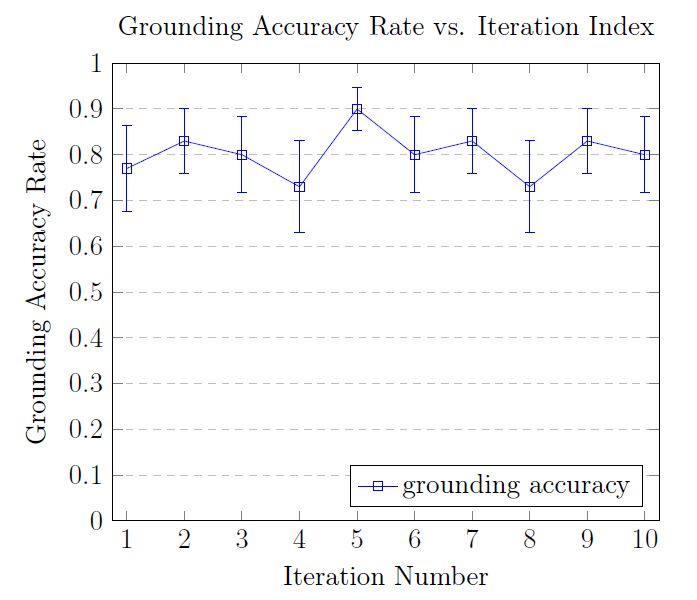
\includegraphics[width=\textwidth]{g_acc}
\caption{Overall grounding accuracy.}
\label{fig:g_acc}
\end{subfigure}
~
\begin{subfigure}[b]{0.50\columnwidth}
\centering
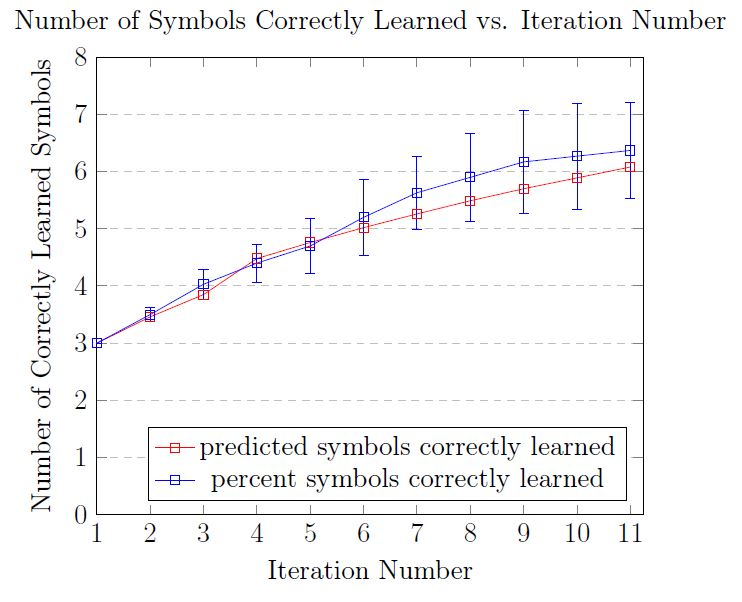
\includegraphics[width=\textwidth]{symbols_corr}
\caption{Number of learned symbols.}
\label{fig:symbols}
\end{subfigure}
\caption{The performance results of the simulation study.}
\end{figure}

\begin{figure}[h]
\centering
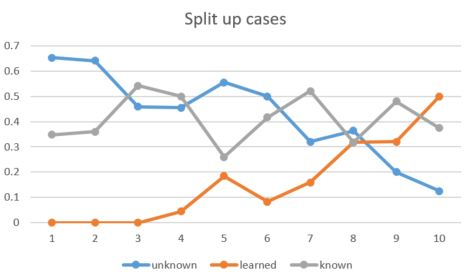
\includegraphics[width=0.7\columnwidth]{learning}
\caption{The percentage of symbols during the simulations.}
\label{fig:g_acc_split}
\end{figure}


%\begin{figure}[h]
%\centering
%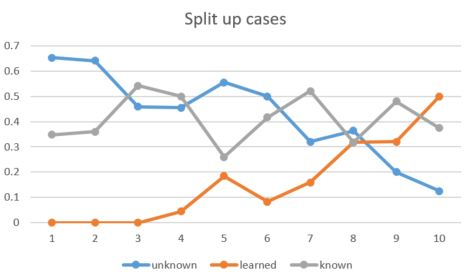
\includegraphics[width=8.5cm]{learning}
%\caption{this is split up (must replot well)}
%\label{fig:g_acc_split}
%\end{figure}


\subsection{Learned Symbols}
In order to better examine the learning behavior exhibited by the DCG-UPUP-Away model, the other performance metric considered is the number of correctly known symbols. Note that the symbols may be incorrectly learned by associating a phrase with the wrong sort of object due to the nature of unsupervised learning.
Initially, the turtlebot is trained with cubes, spheres, and cylinders, but the genrated environments may contain up to 5 additional object types (i.e., fire hydrants, drills, mailboxes, door handles, and traffic cones).
Whenever an unknown phrase is grounded to such an unknown object, the turtlebot learns the new symbol.
Thus, one may calculate the expected number of known symbols as a function of the iteration number using combinatorics to count how many unknown objects are present.
The recorded number of correctly learned symbols are plotted in Fig.~\ref{fig:symbols} in blue, as well as the expected number in red.
%\begin{figure}[h]
%\centering
%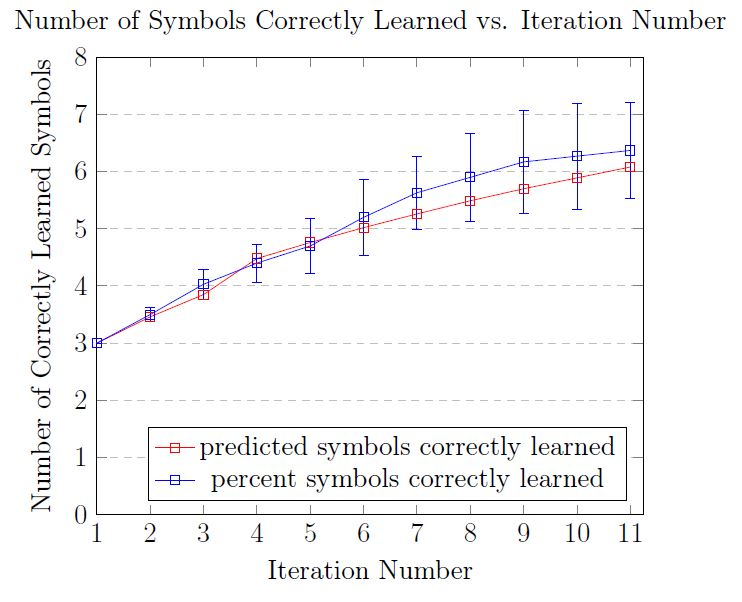
\includegraphics[width=8.5cm]{symbols_corr}
%\caption{this is how we show that we learn symbols. I will update this label (and caption) of this figure. also must use std error bars instead of variance}
%\label{fig:symbols}
%\end{figure}
%(Asking for advice: the x axis ranges from 1 to 11 because I can retrain after the 10th iteration and increase the mean number of symbols learned. It's a small increase, though, so I wouldn't be too upset cutting off the 11th iteration, though.)

As expected, the blue curve starts at $3$ (for the cube, sphere, and cylinder), and stochastically monotonically increases.
In $10\%$ of trials, all $8$ symbols were correctly learned. In other trials the DCG-UPUP-Away model incorrectly grounded unknown phrases (and therefore learned an incorrect symbol) or the 10 iterations collectively never referred to the five initially unknown objects, preventing the DCG-UPUP-Away model from ever learning the new symbol.
Furthermore, learning symbols correctly improves the grounding accuracy: for each additional correctly learned symbol, the turtlebot is over $4\%$ more likely to correctly ground a command. %(TODO generate p values via ANOVA.)

\subsection{Hardware Demonstration}
In addition to the simulation studies, the DCG-UPUP-Away model was tested on an actual turtlebot in a laboratory setting.
The turtlebot was placed facing %a cylinder (known) and 
a cone (unknown).
In addition, a cube (known) and a crate (unknown) were located behind the turtlebot.
All objects were labeled with the AR-track tags \cite{olson2011}, which were used to generate the world model $\Upsilon$ from a kinect camera mounted on the turtlebot.

%I'd like to add a footnote saying that I have videos of these demos
Three natural language commands were used to demonstrate all capabilities of the DCG-UPUP-Away model.
%First, the turtlebot was given the command ``move towards the cube.''
%The turtlebot successfully drove to the cube, demonstrating a correct grounding to a known, perceived object.\\
First, the turtlebot was given the command ``move towards the cone.''
The turtlebot drove to the cone, demonstrating that it perceived the cone as unknown, recognized the phrase ``cone'' as unknown, and grounded the unknown phrase to the unknown object.
Thus, a command was correctly grounded to an unknown perceived object as illustrated in Fig.~\ref{fig:cone}.
Second, the turtlebot was given the command ``move towards the cube.''
The turtlebot rotated in place until the cube came in perception, and then approached the cube.
In other words, the command was first grounded to a known hypothesized object, and then it was grounded to a known perceived object once the cube was seen. 
Finally, the turtlebot was given the command ``move towards the crate.''
Once again, the turtlebot explored its surrounding by rotating at its current location and drove to the crate once it perceived it (as illustrated in Fig.~\ref{fig:crate}). %rotated in place, this time until it saw the crate, whereupon it drove to the crate.
The experimental results demonstrate two important behaviors: 1) the turtlebot must have learned what a cone was, otherwise the unknown phrase (``crate'') would have been grounded to the cone, and 2) the turtlebot grounded the command to an unknown hypothesized object until the crate was perceived. The interested reader is referred to the following link \footnote{https://www.youtube.com/playlist?list=PL8sYMUToK9s6dAu3qMHHOef8FyhOnDK4E} for the videos corresponding to these experiments.
%The execution of this last command, including images of the physical behavior of the turtlebot as well as the model used for grounding, is shown in Figure~\ref{fig:hardware_demo}.

%\begin{figure}[ht]
%\centering
%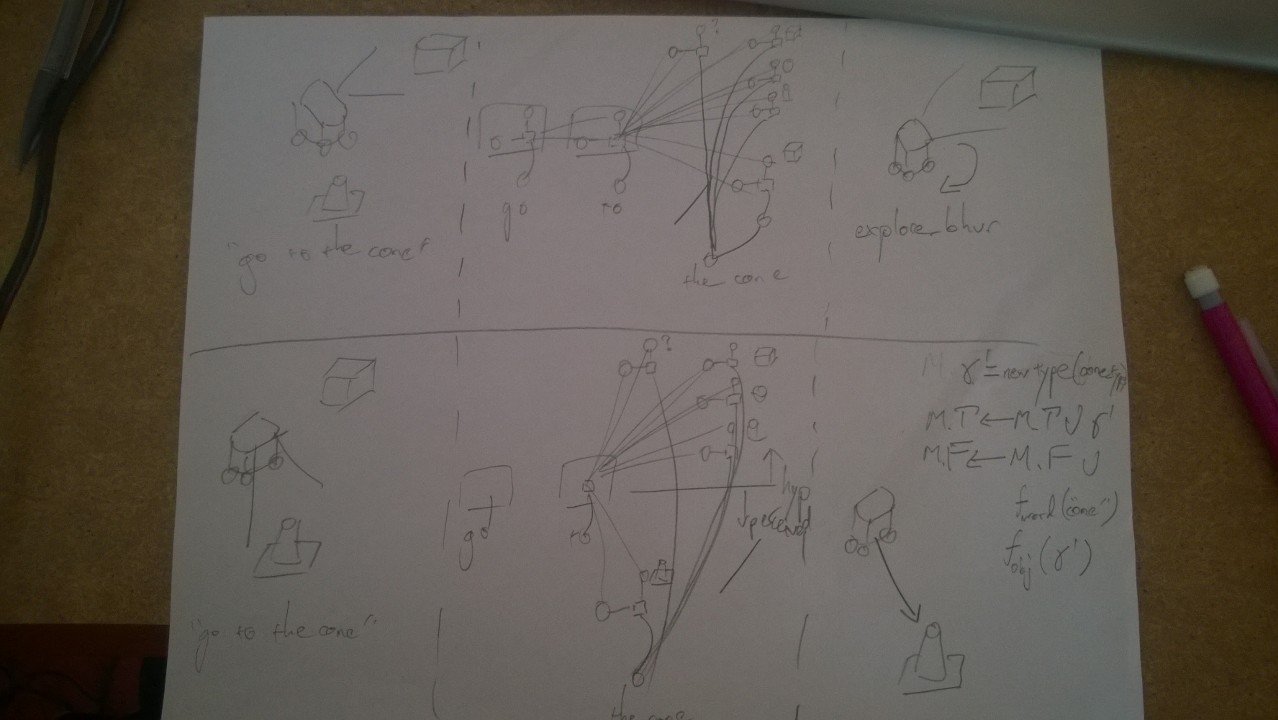
\includegraphics[width=8.5cm]{hardware_sketch}
%\caption{this is a sketch of the 6 subfigures that demonstrate hypothesized groundings on hardware and in the model, and shows how it learns. I'd like this to go across the top of the page.}
%\label{fig:hardware_demo}
%\end{figure}
%\begin{figure*}
%\begin{subfigure}[b]{0.31\textwidth}
%\centering
%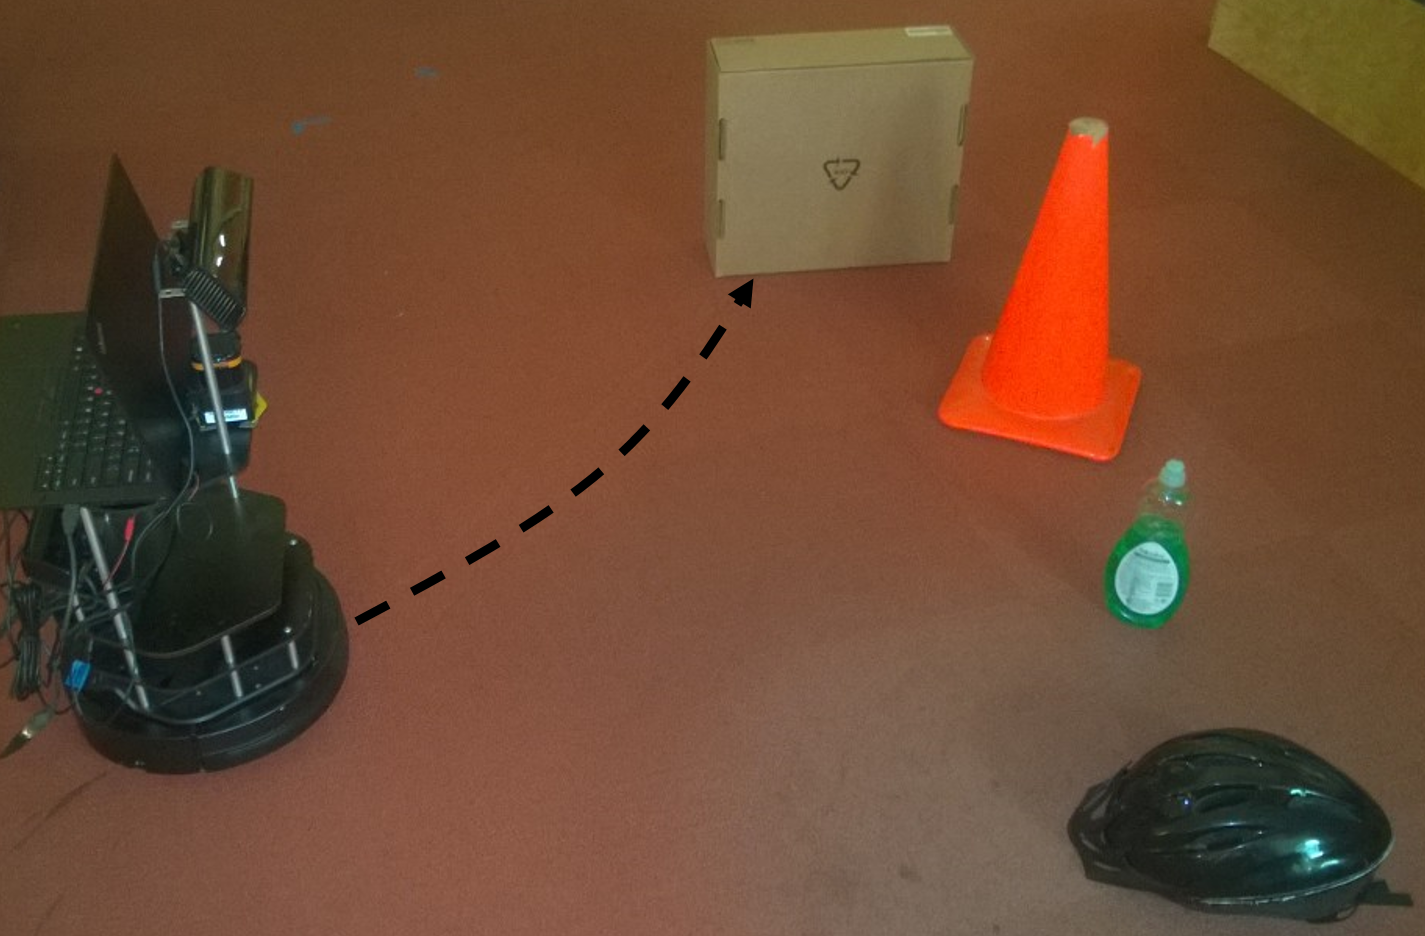
\includegraphics[width=\textwidth]{hardware1.png}
%\caption{The command ``move towards the box" is given, and the turtlebot approaches the box by grounding a known phrase to a known object.}
%\label{fig:g_acc}
%\end{subfigure}
%~
%\begin{subfigure}[b]{0.295\textwidth}
%\centering
%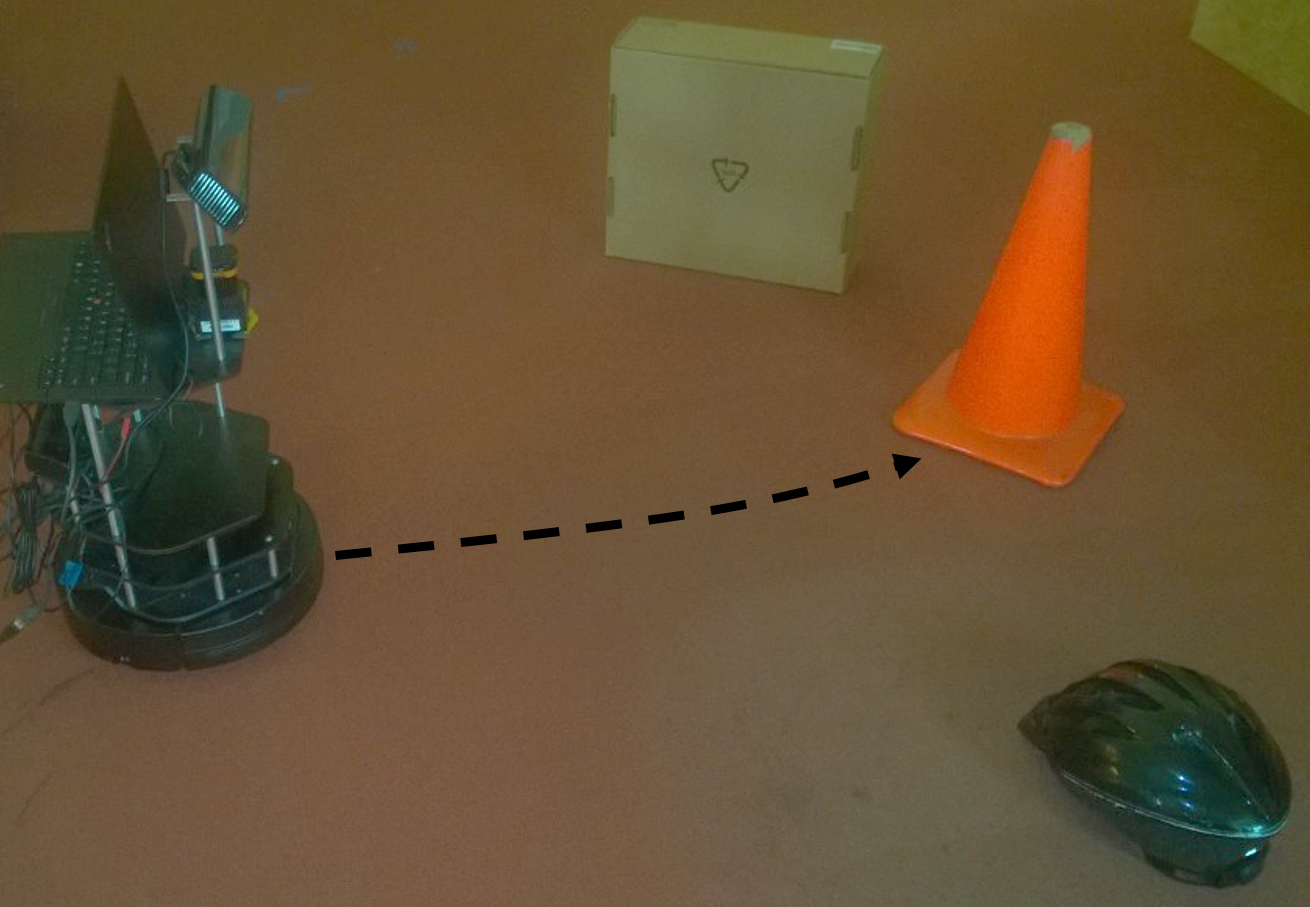
\includegraphics[width=\textwidth]{hardware2.png}
%\caption{The command ``move towards the cone" is given, and the turtlebot drives to the cone because unknown phrase ``cone" is grounded to the unknown object cone.}
%\label{fig:symbols}
%\end{subfigure}
%~
%\begin{subfigure}[b]{0.355\textwidth}
%\centering
%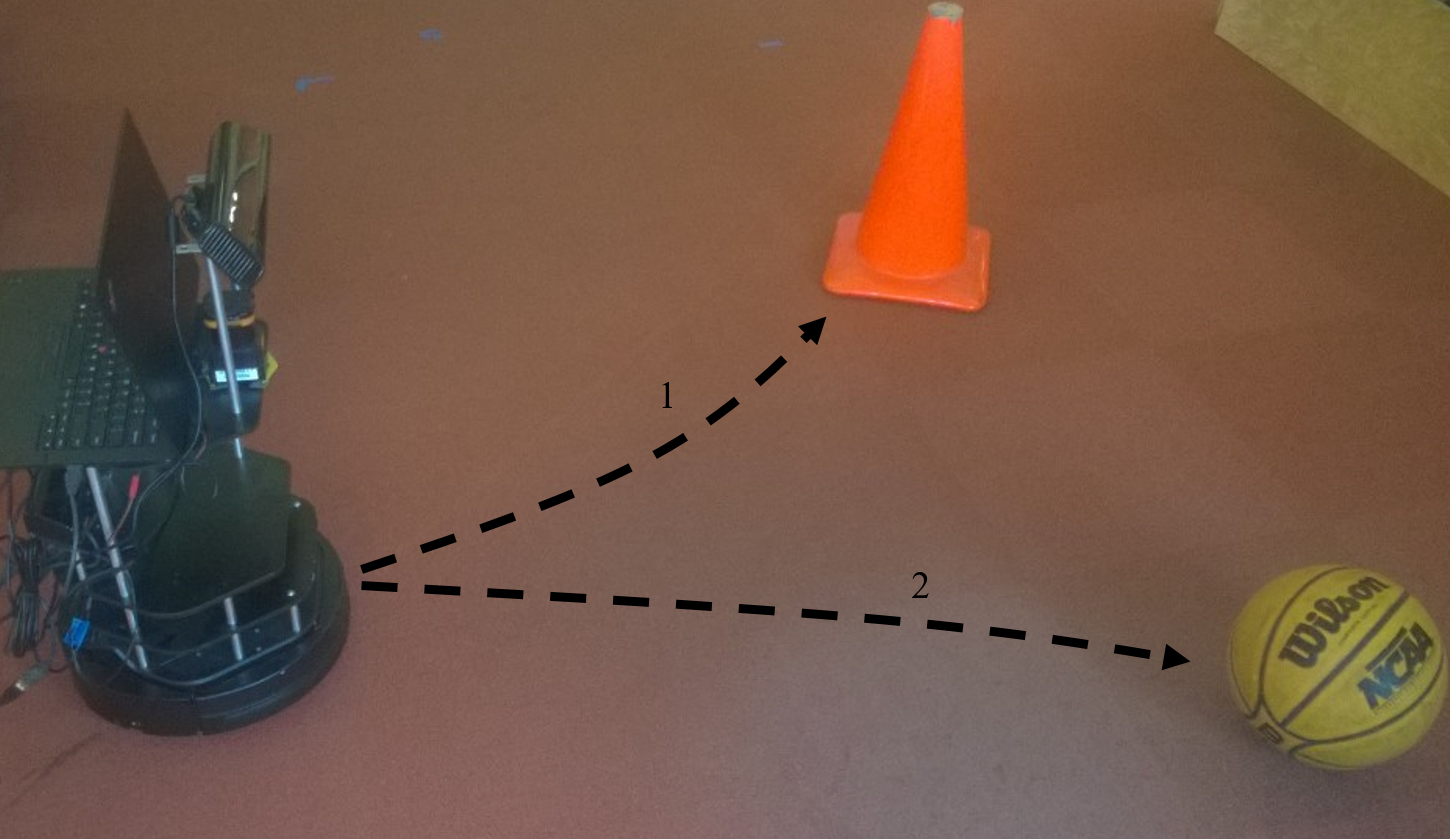
\includegraphics[width=\textwidth]{hardware3.png}
%\caption{The command ``move towards the cone" is given and the turtlebot follows path 1. The command ``move towards the ball" is given, and the turtlebot follows path 2.}
%\label{fig:g_acc_split}
%\end{subfigure}
%\caption{Some illustrations of iterative learning via the proposed model. (a) The turtlebot initially knows a box, a helmet, and a soap box, then (b) it learns what a cone is, and then (c) it learns what a ball is.}
%\end{figure*}


\begin{figure}
\begin{subfigure}[b]{0.305\columnwidth}
\centering
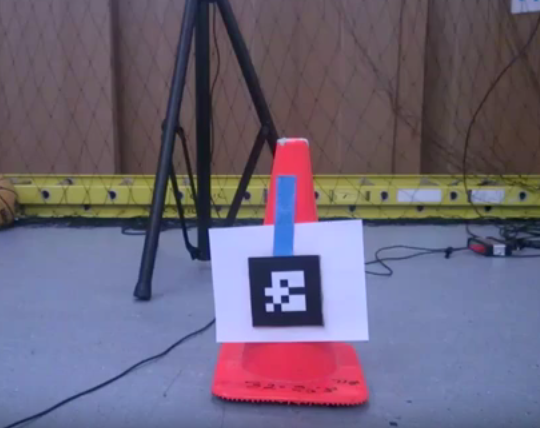
\includegraphics[width=\textwidth]{c1.png}
\caption{t= 0 sec.}
\label{fig:g_acc}
\end{subfigure}
~
\begin{subfigure}[b]{0.31\columnwidth}
\centering
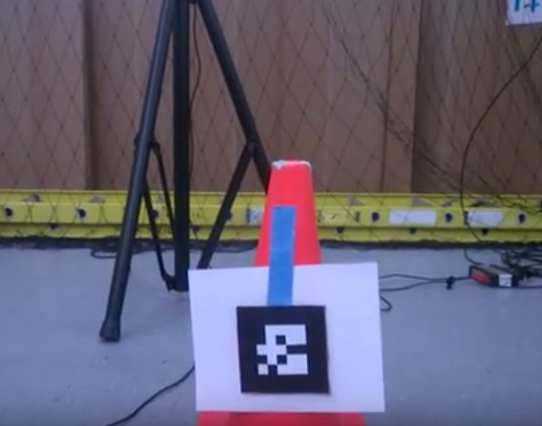
\includegraphics[width=\textwidth]{c2.png}
\caption{t= 45 sec.}
\label{fig:symbols}
\end{subfigure}
~
\begin{subfigure}[b]{0.315\columnwidth}
\centering
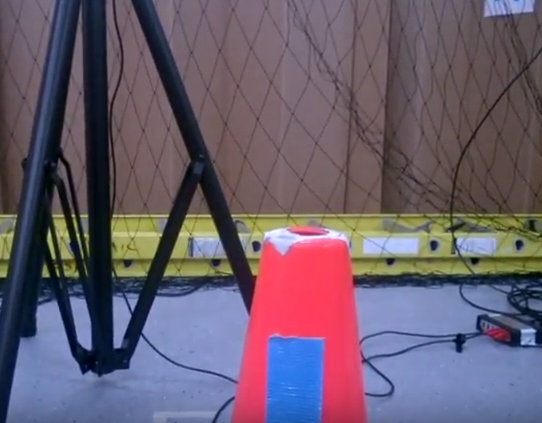
\includegraphics[width=\textwidth]{c3.png}
\caption{t= 50 sec.}
\label{fig:g_acc_split}
\end{subfigure}
\caption{An illustration of learning new symbol. The turtlebot initially does not know what a cone is, a command is given as ``move towards the cone". (a) Since there is an unknown object in its perceived world, it grounds the unknown phrase ``cone" to the unknown object, (b,c) it drives to the cone.}
\label{fig:cone}
\end{figure}

\begin{figure*}
\begin{subfigure}[b]{0.15\textwidth}
\centering
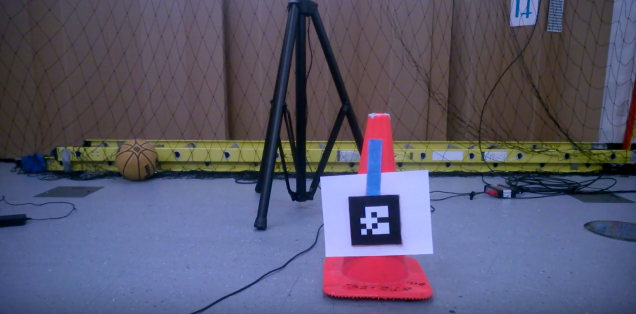
\includegraphics[width=\textwidth]{1.png}
\caption{t=0 sec.}
\label{fig:g_acc}
\end{subfigure}
~
\begin{subfigure}[b]{0.15\textwidth}
\centering
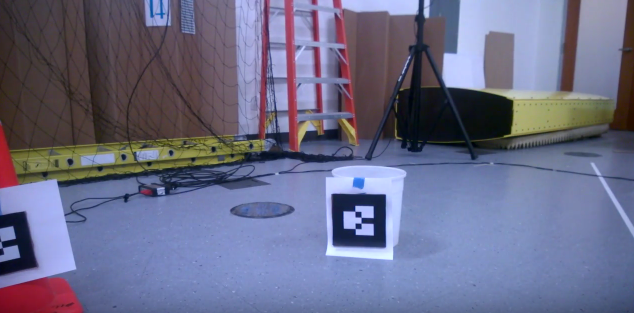
\includegraphics[width=\textwidth]{2.png}
\caption{t=25 sec.}
\label{fig:symbols}
\end{subfigure}
~
\begin{subfigure}[b]{0.15\textwidth}
\centering
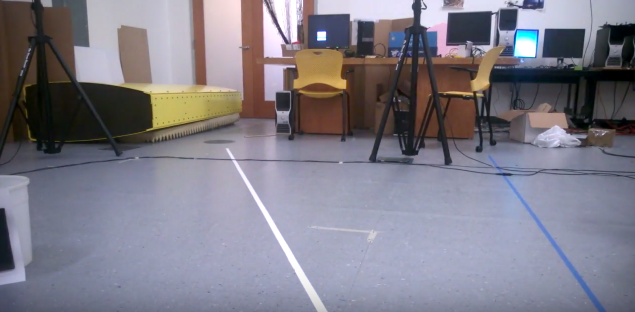
\includegraphics[width=\textwidth]{3.png}
\caption{t=50 sec.}
\label{fig:g_acc_split}
\end{subfigure}
~
\begin{subfigure}[b]{0.15\textwidth}
\centering
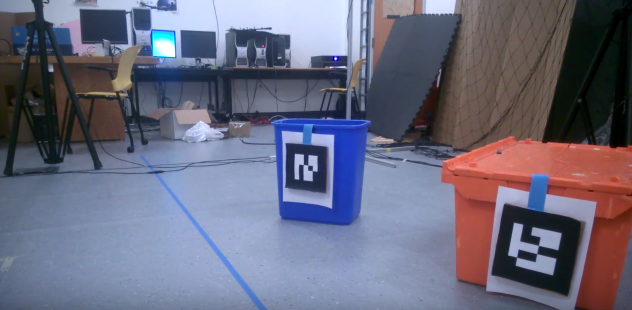
\includegraphics[width=\textwidth]{4.png}
\caption{t=70 sec.}
\label{fig:g_acc}
\end{subfigure}
~
\begin{subfigure}[b]{0.15\textwidth}
\centering
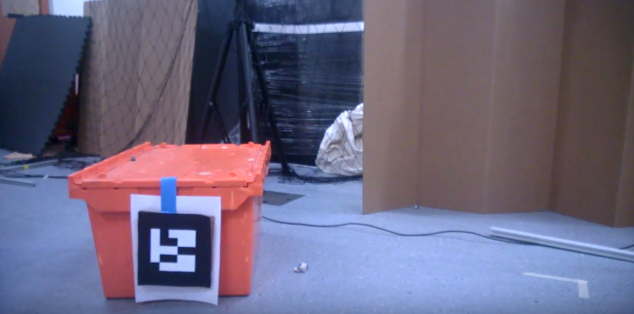
\includegraphics[width=\textwidth]{5.png}
\caption{t=95 sec.}
\label{fig:symbols}
\end{subfigure}
~
\begin{subfigure}[b]{0.15\textwidth}
\centering
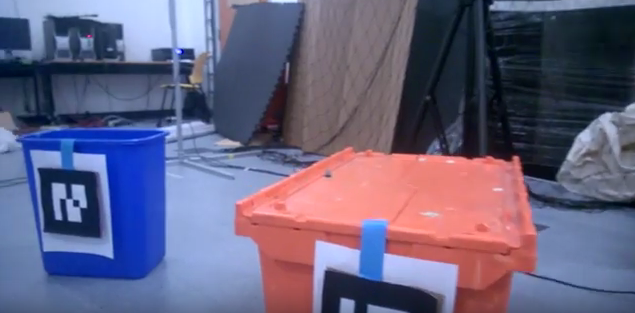
\includegraphics[width=\textwidth]{6.png}
\caption{t=120 sec. }
\label{fig:g_acc_split}
\end{subfigure}
\caption{An illustration of grounding to a hypothetical object. The robot initially knows all objects in the world other than a crate. The turtlebot is given a command as ``move towards the crate". (a) First, it does not see an unknown object in its perceived world so it creates a hypothetical unknown object, (b,c,d) it explores the world by rotating at its current location until it perceives an unknown object, (e) It perceives an unknown object and grounds to it, (f) it drives to the crate.}
\label{fig:crate}
\end{figure*}


\subsection{Limitations}
The previous sections demonstrated that the proposed model DCG-UPUP-Away results in the successful execution of various natural language commands. This section discusses the main limitations of the model.
%of the DCG-UPUP-Away model encountrduring  are equally important in characterizing the limits of its performance.\\
In particular, the most obvious limitation of the DCG-UPUP-Away model is the assumption of referring an unknown phrase to the first perceived unknown object. %that, in the absence of additional information, unknown phrases refer to the first perceived unknown object.
One strategy to relax this assumption has been explored in Section~\ref{sec:color} by associating language adjectives with object properties. However, a more sophisticated strategy is required for generalizable solutions.  %have been explored in Section (TODO color section), but so far only a relatively simple method has been used.\\
Moreover, the DCG-UPUP-Away model assumes a one-to-one correspondence between unknown phrases and unknown objects; thus it cannot, for example, learn synonyms by grounding unknown phrases to the known object types.